% Standard Article Definition
\documentclass[]{article}

% Page Formatting
\usepackage[margin=1in]{geometry}
\setlength\parindent{0pt}

% Graphics
\usepackage{graphicx}

% Math Packages
\usepackage{physics}
\usepackage{amsmath, amsfonts, amssymb, amsthm}
\usepackage{mathtools}

% Extra Packages
\usepackage{pdfpages}
\usepackage{hyperref}
% \usepackage{listings}

% Section Heading Settings
\usepackage{enumitem}
% \renewcommand{\theenumi}{\alph{enumi}}
\renewcommand*{\thesection}{Problem \arabic{section}}
\renewcommand*{\thesubsection}{\alph{subsection})}
\renewcommand*{\thesubsubsection}{}%\quad \quad \roman{subsubsection})}

\newcommand{\Problem}{\subsubsection*{\textbf{PROBLEM:}}}
\newcommand{\Solution}{\subsubsection*{\textbf{SOLUTION:}}}
\newcommand{\Preliminaries}{\subsubsection*{\textbf{PRELIMINARIES:}}}

%Custom Commands
\newcommand{\N}{\mathbb{N}}
\newcommand{\Z}{\mathbb{Z}}
\newcommand{\Q}{\mathbb{Q}}
\newcommand{\R}{\mathbb{R}}
\newcommand{\C}{\mathbb{C}}

\newcommand{\SigAlg}{\mathcal{S}}

\newcommand{\Rel}{\mathcal{R}}

% \newcommand{\toI}{\xrightarrow{\textsf{\tiny I}}}
% \newcommand{\toS}{\xrightarrow{\textsf{\tiny S}}}
% \newcommand{\toB}{\xrightarrow{\textsf{\tiny B}}}

\newcommand{\divisible}{ \ \vdots \ }
\newcommand{\st}{\ : \ }

% Theorem Definition
\newtheorem{definition}{Definition}
\newtheorem{assumption}{Assumption}
\newtheorem{theorem}{Theorem}
\newtheorem{lemma}{Lemma}
\newtheorem{proposition}{Proposition}
\newtheorem{remark}{Remark}
% \newtheorem{example}{Example}
% \newtheorem{counterExample}{Counter Example}


%opening
\title{MATH 6301 Real Analysis I \\ Homework 4}
\author{Jonas Wagner\\ jonas.wagner@utdallas.edu}
\date{2022, October 27\textsuperscript{th}}

\begin{document}

\maketitle

\tableofcontents

\includepdf[pages={2}]{math6301a4-2022.pdf}

% Problem 1 ----------------------------------------------
\newpage
\section{}
\Problem
Assume that $U \subset \R^n$ is an open set and $f \st U \to \R$ is a differentiable function.
Show that for every $k = 1,2,\dots,n$, the partial derivative \[
    \pdv{f}{x_k} \st U \to \R
\] is $\mathcal{B}_n$-measurable (here $\mathcal{B}_n$ stands for the $\sigma$-algebra of Borel sets in $\R^n$).

\Preliminaries
\begin{definition}
    Let $\SigAlg \subset P(X)$ is a $\sigma$-algebra and $E \in \SigAlg$.
    The function $f : E \to \overline{\R}$ is called \emph{\underline{measurable}} relative to $\SigAlg$ (i.e. $\SigAlg$-measurable) iff \[
        \forall_{a \in \R} f^{-1}(a,\infty] := \{x \in E \st f(x) > a\} \in \SigAlg
    \] 
\end{definition}
\begin{remark}
    Assume that $f : E \to \overline{\R}$, $E \in \SigAlg \subset P(X)$ is $\SigAlg$-measurable.
    Then the following are also $\SigAlg$-measurable
    \begin{enumerate}
        \item $f^2 : E \to \overline{R}$
        \item $\abs{f} : E \to \overline{R}$
        \item $\frac{1}{f} : E \to \overline{R}$
        \item $a \cdot f : E \to \overline{R}, \ a \in \R$
    \end{enumerate}
\end{remark}

\Solution


% Problem 2 ----------------------------------------------
\newpage
\section{}
\Problem


\Preliminaries



\Solution




% Problem 3 ----------------------------------------------
\newpage
\section{}
\Problem



\Preliminaries


\Solution




% Problem 4 ----------------------------------------------
\newpage
\section{}
\Problem



\Preliminaries


\Solution




% Problem 5 ----------------------------------------------
\newpage
\section{}
\Problem


% \Preliminaries

\Solution










\end{document}
